\subsection{K-Means}
We have tested on each dataset 57 different configurations of the K-Means algorithm, by using the 3 different distance metrics with 19 different values of the k (from 2 to 20). For each of these configurations, we have run the K-Means 10 times, in order to account for the randomness of the centroid initialization. This results in a total of 570 runs of the K-Means algorithm for each dataset. From the evaluation metrics extracted for each of these runs, we study the effect of each of the 2 hyperparameters and achieve conclusions about them through statistical analysis.

\subsubsection{Preliminary Study}
Before starting with the more rigorous statistical analysis, let us first observe some preliminary patterns about the measured metrics and the effect of each hyperparameter on the clustering performance.

In Figure \ref{fig:metrics_corr} we summarize the relationship between the different metrics that were measured. It is a matrix plot where the lower triangle is a heatmap of the Pearson correlations between each pair of metrics, the diagonal elements are the histogram distributions of values of each metric, and the upper triangular has for each pair of metrics the plot of their values for all runs. It is interesting to observe that, while we would expect all of the metrics to agree on the identified trends, there are some cases where the opposite behaviour is displayed. An example of this is the negative correlation between E (total variance) and DBI (Davies-Bouldin Index): since the DBI measures cluster compactness, we would expect it to directly correlate to E; however, we observe that there is a negative correlation between them. This specific figure was extracted from the results on the Mushroom dataset, but the conclusions are the same for the others (the plots can be found in the \texttt{code} floder).

\begin{figure}[h]
    \centering
    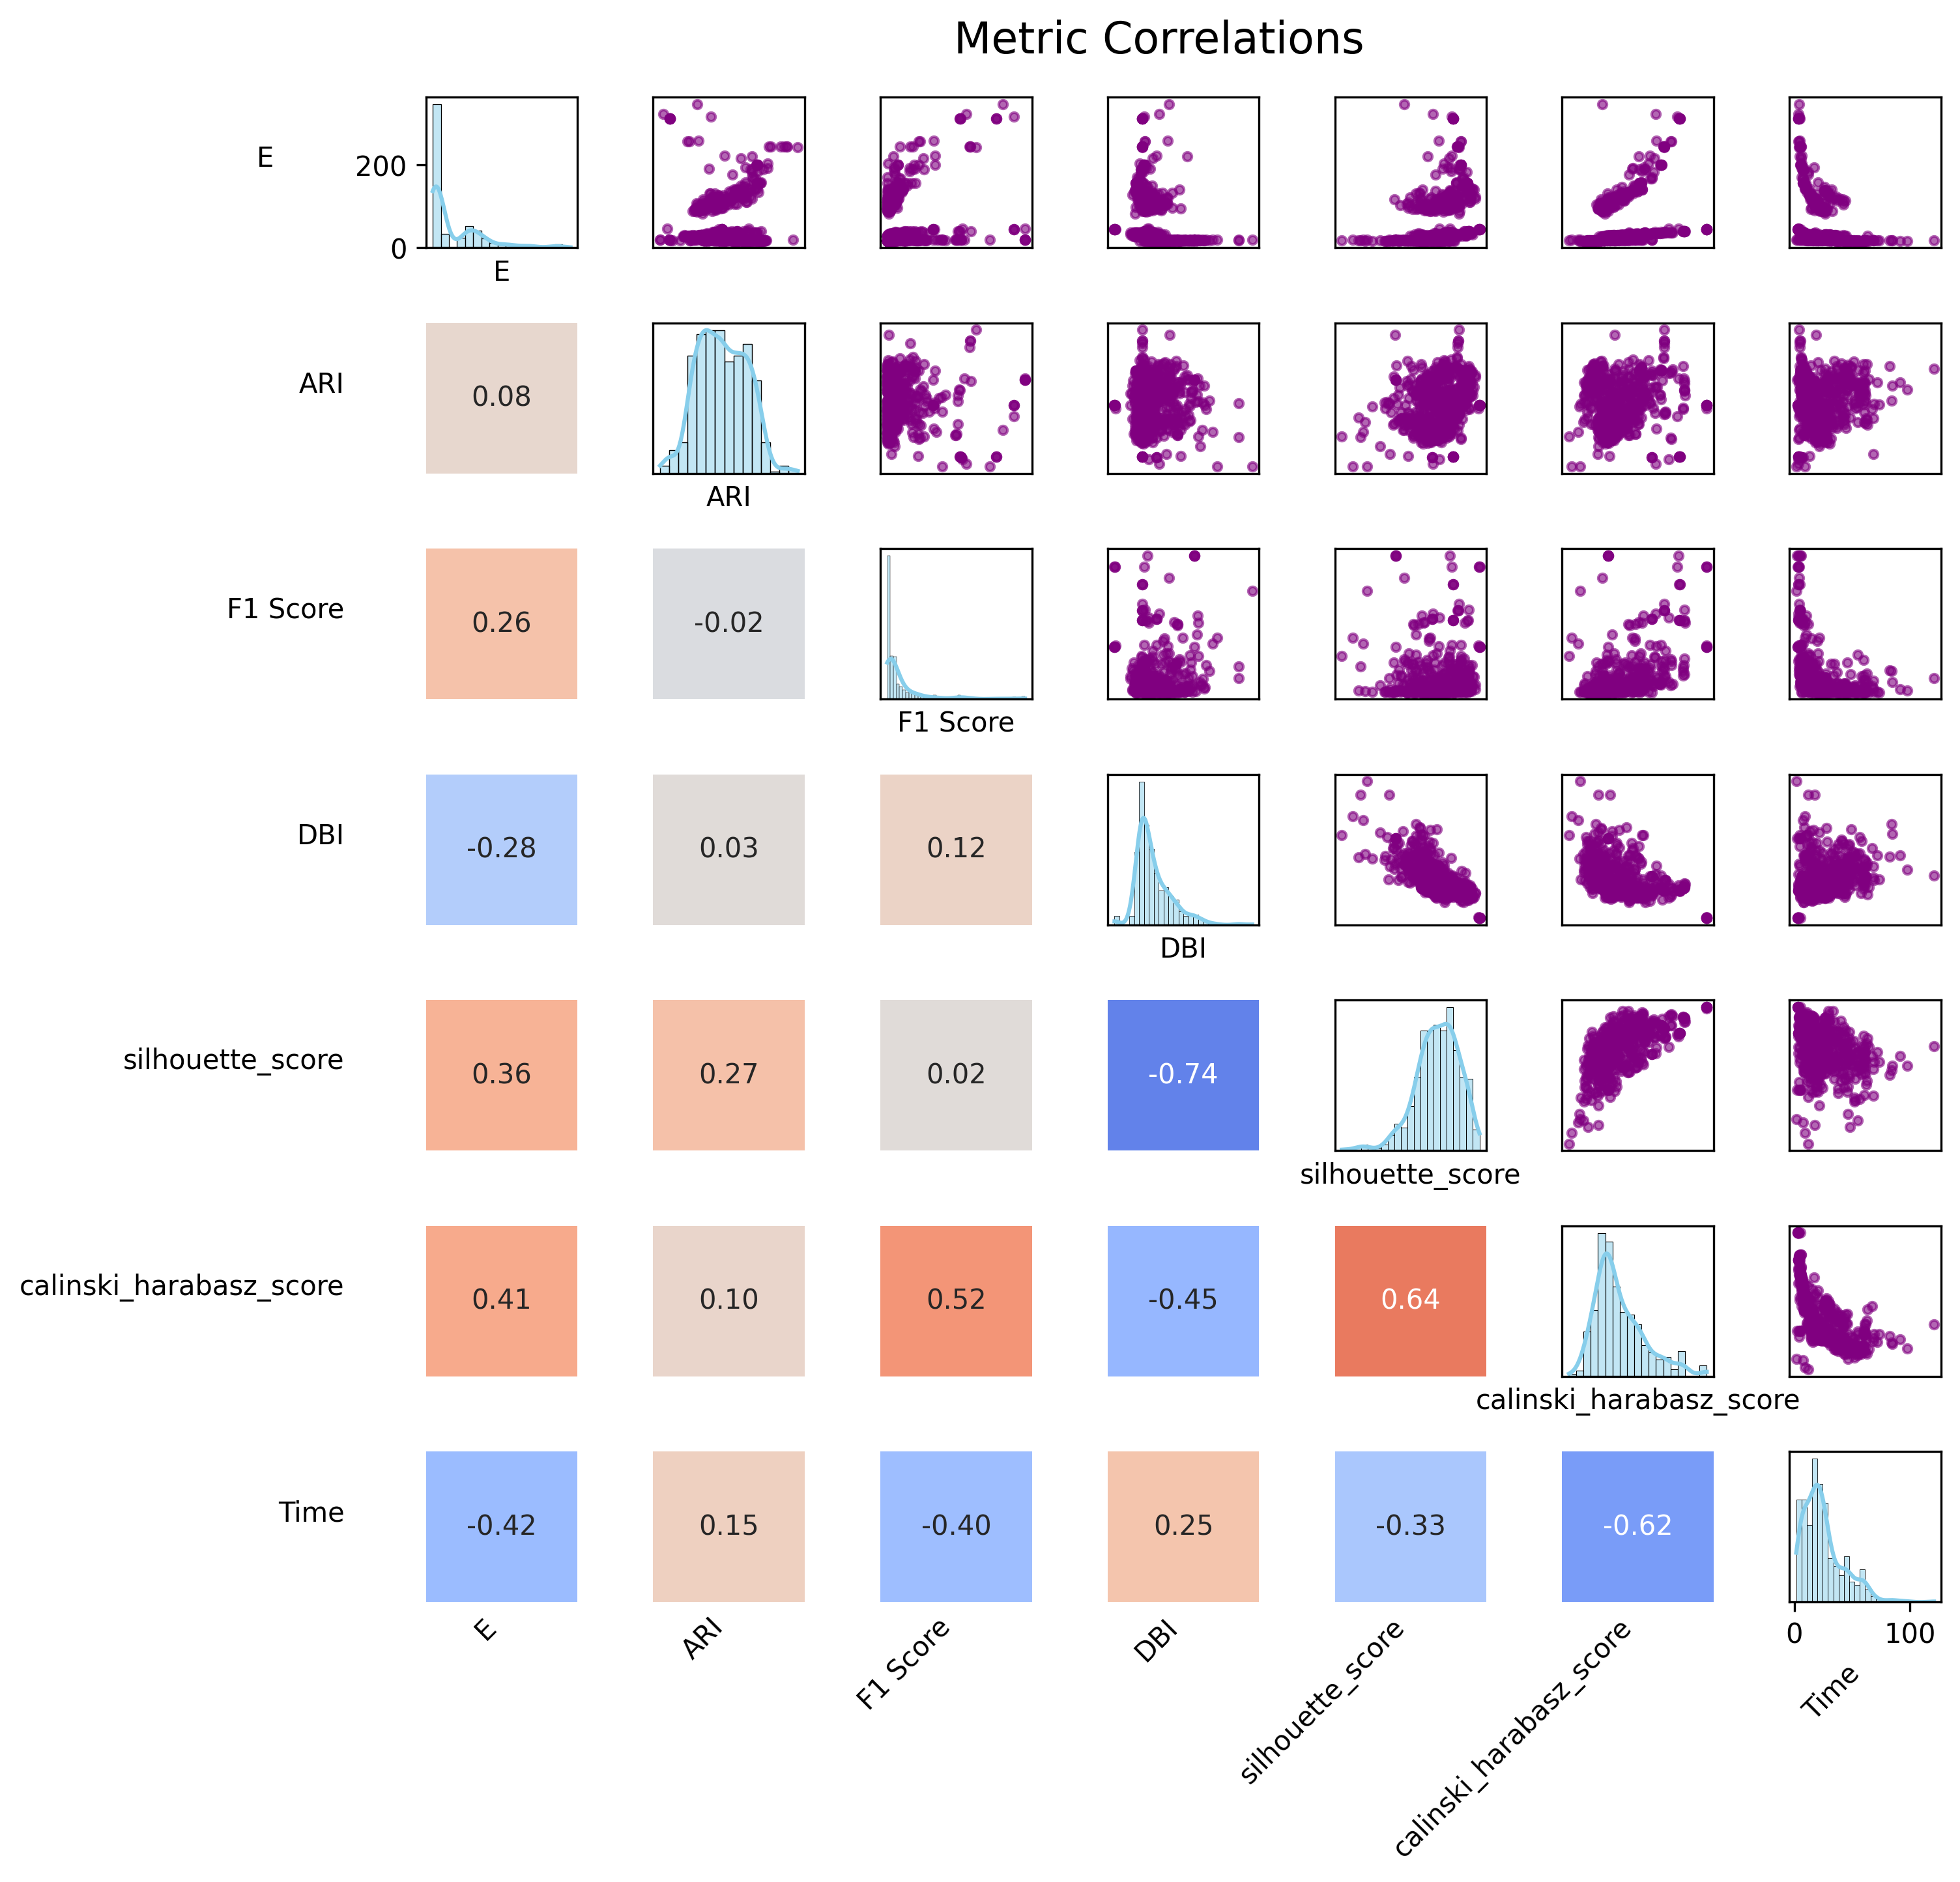
\includegraphics[width=0.7\textwidth]{figures/metrics_correlations_matrix.png}
    \caption{Metrics correlations summary}
    \label{fig:metrics_corr}
\end{figure}

Parallelly, a different set of interesting relationship are displayed in Figure \ref{fig:pairplot}, where we can see heatmaps of the F1 Score and the Time across the different pairwise hyperparameter configurations. We can observe a general trend regarding execution time: it seems to have considerably larger values for the Clark distance metric compared to those of the other 2, which reflects the higher computational cost that this distance metric has. Additionally, we see a noteworthy divergence in the F1 Score trends with respect to the values of k: in the Mushroom dataset (which has 2 classes), lower values of k seem to achieve a better F1 Score; meanwhile, in the Pen-based dataset (which has 10 classes), intermediate values of k (between 7 and 11) seem to achieve the best scores. This was to be expected, yet it still is compelling to see it reflected so clearly in the results. 

\begin{figure}[H]
    \centering
    \begin{subfigure}{0.49\textwidth}
        \centering
        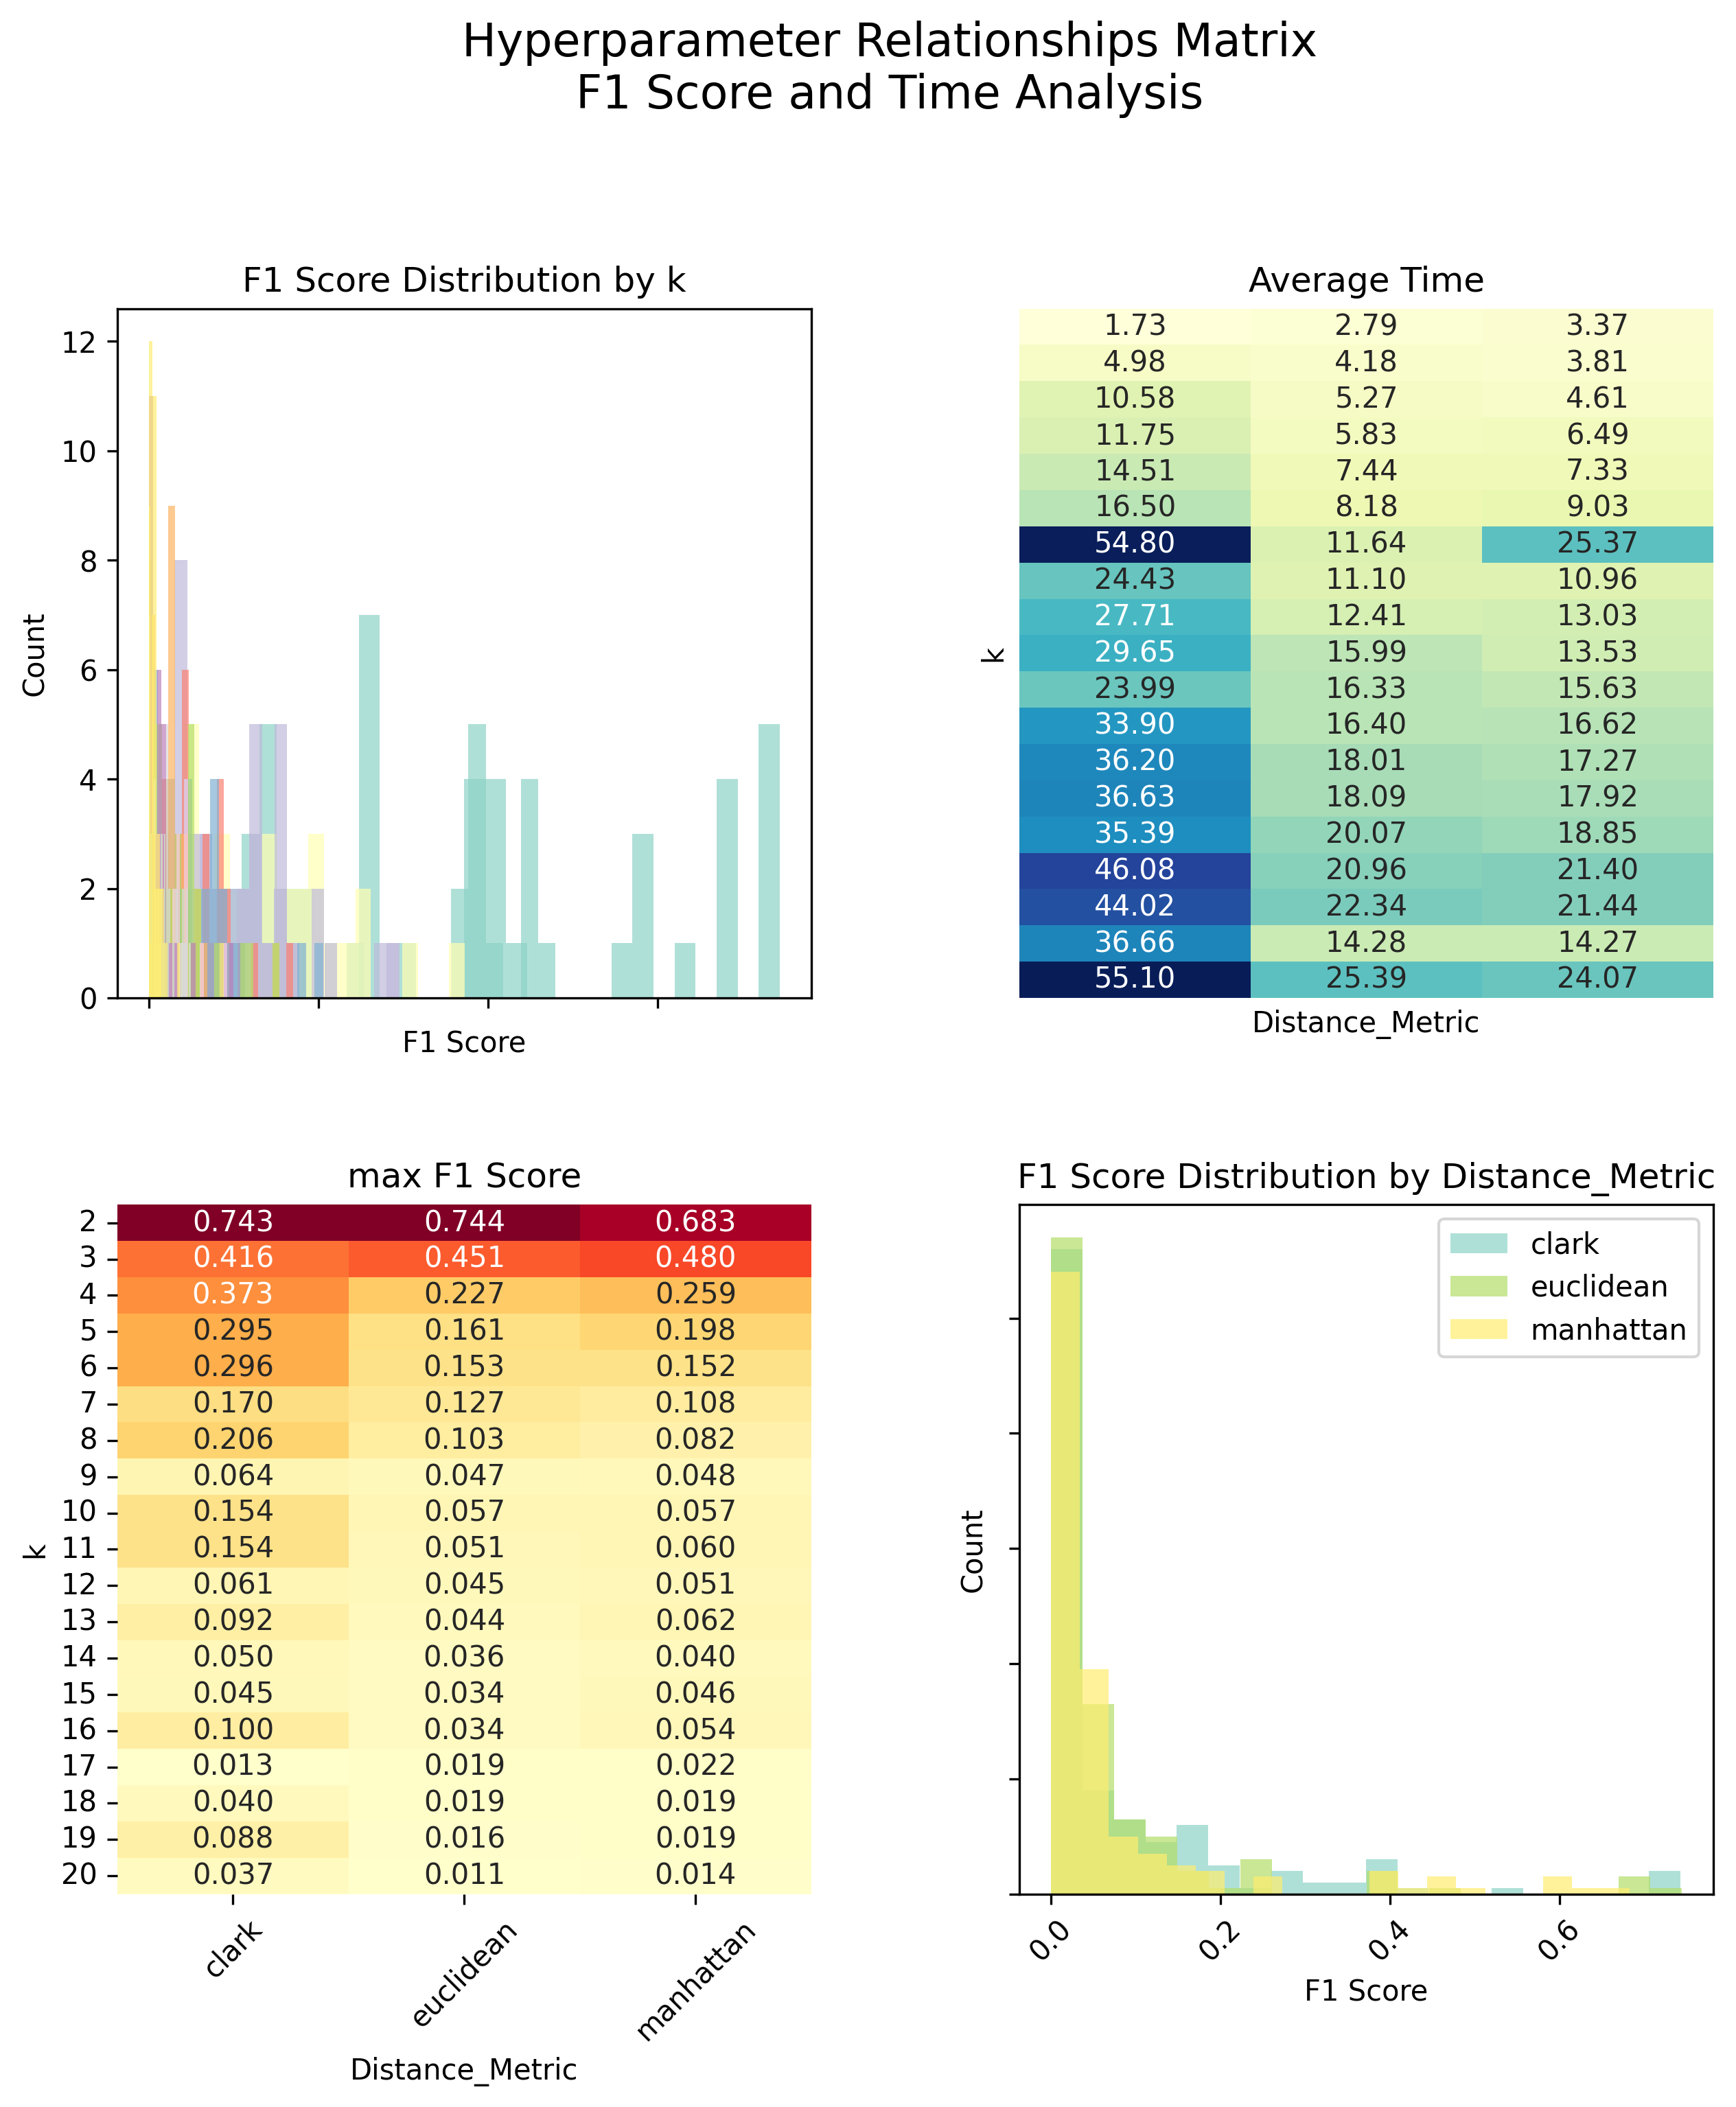
\includegraphics[width=\linewidth]{figures/mushroom_hyperparameter_pairplot_matrix.png}
        \caption{Mushroom pairplot matrix}
    \end{subfigure}
    \hfill
    \begin{subfigure}{0.49\textwidth}
        \centering
        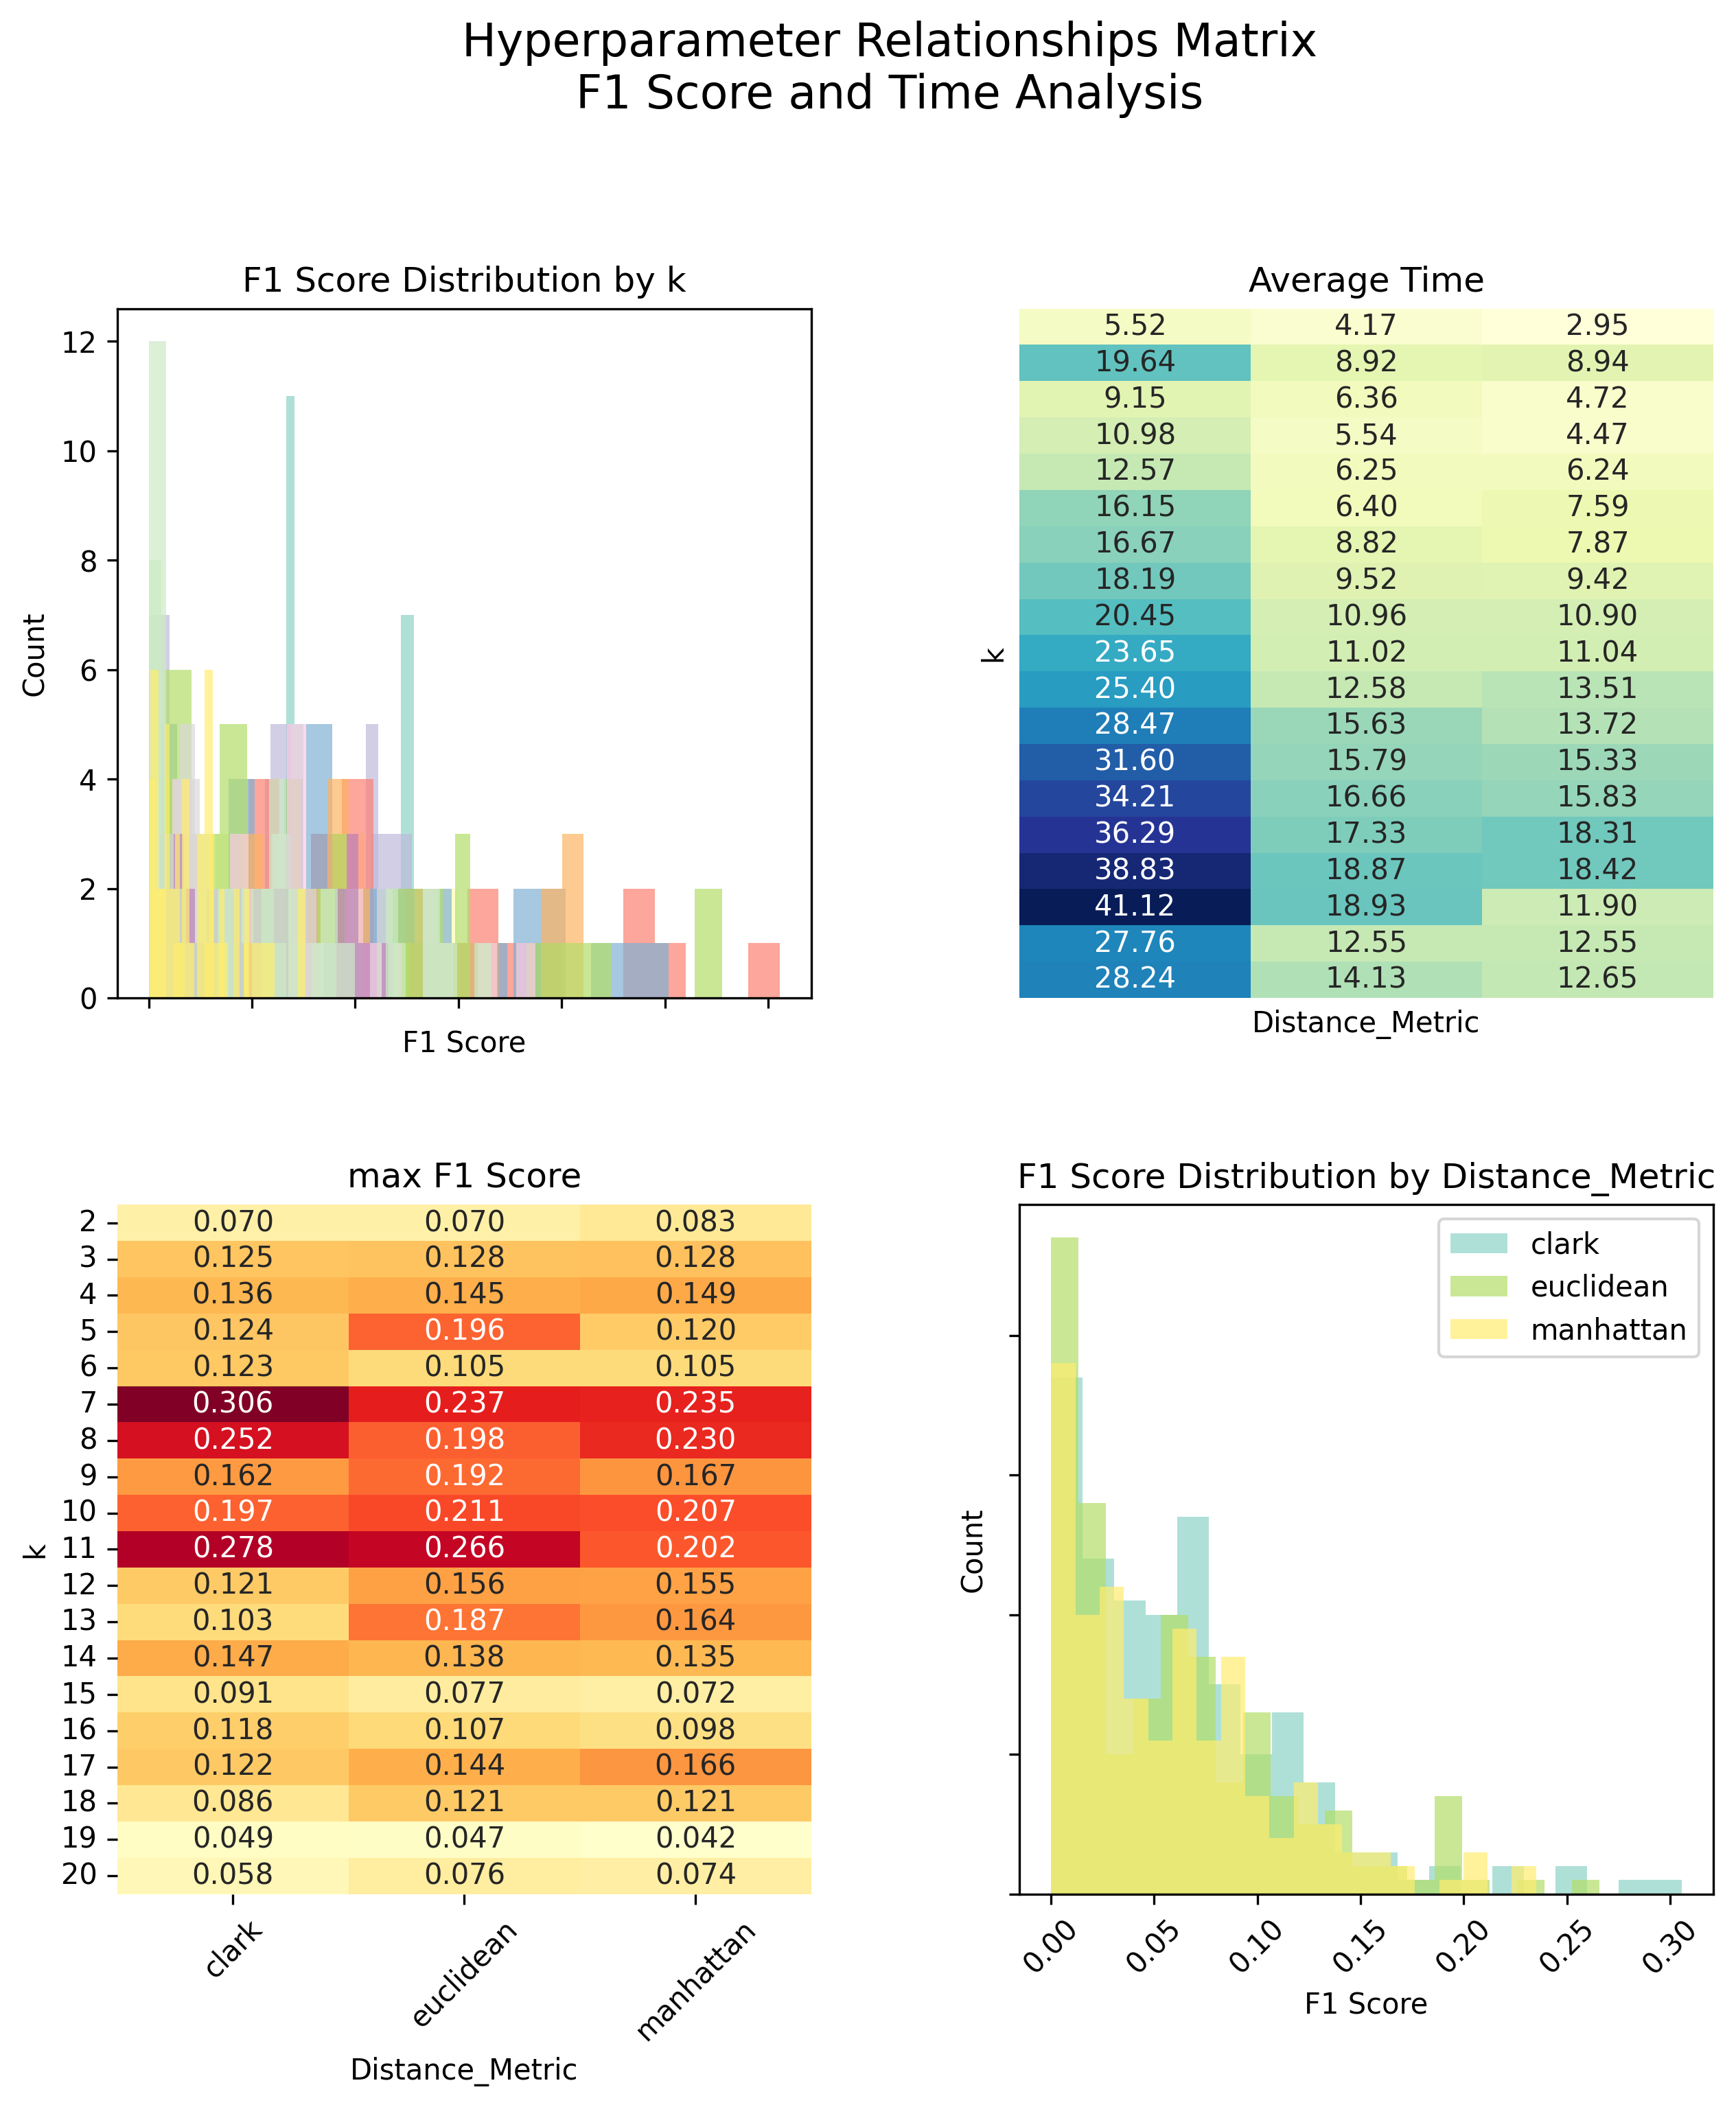
\includegraphics[width=\linewidth]{figures/penbased_hyperparameter_pairplot_matrix.png}
        \caption{Pen-based pairplot matrix}
    \end{subfigure}
    \caption{Hyperparameter pairplot matrices based on F1 Score and Time}
    \label{fig:pairplot}
\end{figure}

\subsubsection{Statistical Analysis}
For the statistical analysis, we have first performed Friedman tests to determine if there are significant differences in each of the metrics among the different possible values of each hyperparameter. With a confidence level of $\alpha = 0.15$, all of the metrics agree across all 3 datasets that \textbf{there are significant differences} when varying across values of k, and also when changing the distance metric. 

\textit{Note:} Due to the vast amount of statistical results extracted, not all of them will be displayed; only the most relevant ones will be explicitly highlighted. All of the results can be found in the \texttt{code} folder, inside \texttt{Analysis/plot\_and\_tables/KMeansReports}, for each dataset.

Since we have found significant differences between different values of the hyperparameters, we have then applied post-hoc tests on all of the metrics to find more specifically where these differences lie:
\begin{itemize}
    \item For the k, we have performed Nemenyi tests on each of the 3 datasets.
    \begin{enumerate}
        \item \textbf{Hepatitis:} Most of the metrics agree that the lower values of k show better clustering performance. We observe this in the grouped metric averages, which generally get worse as the k increases. The only exception is the DBI, for which the differences are mostly not significant. For the rest of metrics, k=2 always shows significant differences when compared with k=19 and k=20, for instance. These results make sense, since the Hepatitis dataset has 2 classes.
        \item \textbf{Mushroom:} In this case, there are some metrics that cannot find any case of pairwise significant differences. The two that find the most relevant differences are F1 Score and Calinski-Harabasz score, which in both cases we can see that values of k from 2 to 4 show significantly better clustering performance than values from 12 to 20. Once again, since the Mushroom dataset also has 2 classes, these conclusions were to be expected.
        \item \textbf{Pen-based:} For this dataset, most of the metrics do not identify significant differences among values of k. The only 2 exceptions are ARI and Calinski-Harabasz score: the ARI identifies values 2 through 5 to be significantly worse than those greater than 10, while there are no differences among high values of k; meanwhile, the Calinski-Harabasz score seems to find significant differences between the lowest values (below 5) and the highest values (above 14), favoring the small values. Additionally, by studying the F1 Score averages, we see a clear trend of better performance between values 7 and 10 (though statistically these differences are not meaningful). Overall, these results are not very conclusive, and we only deduce that the K-Means might not be the most appropiate clustering algorithm for the Pen-based dataset.
    \end{enumerate}
    \item For the distance metric, we decided on applying Bonferroni tests instead of Nemenyi, considering the Euclidean distance to be the ``control'' value.
    \begin{enumerate}
        \item \textbf{Hepatitis:} 
        \item \textbf{Mushroom:} 
        \item \textbf{Pen-based:} 
    \end{enumerate}
\end{itemize}
